\subsection{Stability Analysis of the Equilibrium}



Question 2 presents an unstable state in which the population of organism 2 ($N_2$) dominates and reduces the population of organism 1($N_1$) to local extinction. The proposed intervention involved reducing the populations of both $N_1$ and $N_2$ by a constant factor $\rho \in (0,1)$ The question is, is this intervention effective and if so, is there a range of value of $\rho$ in which the intervention is effective? 

More formally the state of the system is represented by a vector 
$$ \textbf{N} = \begin{bmatrix}N_1 \\ N_2\end{bmatrix}$$
The system is an an region of the system that moves towards an equilibrium where $N_1=0$. The question is then: is there some scalar value $\rho$ which results in the system moving towards an equilibirum where $N_1, N_2 > 0$

The result of the reduction reduction by rho is a vector $\textbf{N'}$

$$ \textbf{N'} = \begin{bmatrix}N_1' \\ N_2'\end{bmatrix}$$

Since $\textbf{N}$ is multiplied by a scalar, $\textbf{N'}$ will have the same direction as $\textbf{N}$, but a smaller magnitude. 

From the initial wording of the question we know that $N1$ goes to 0. The region of the phase space for which this is the case is the region in which 


\begin{figure}[h]
  \centering
  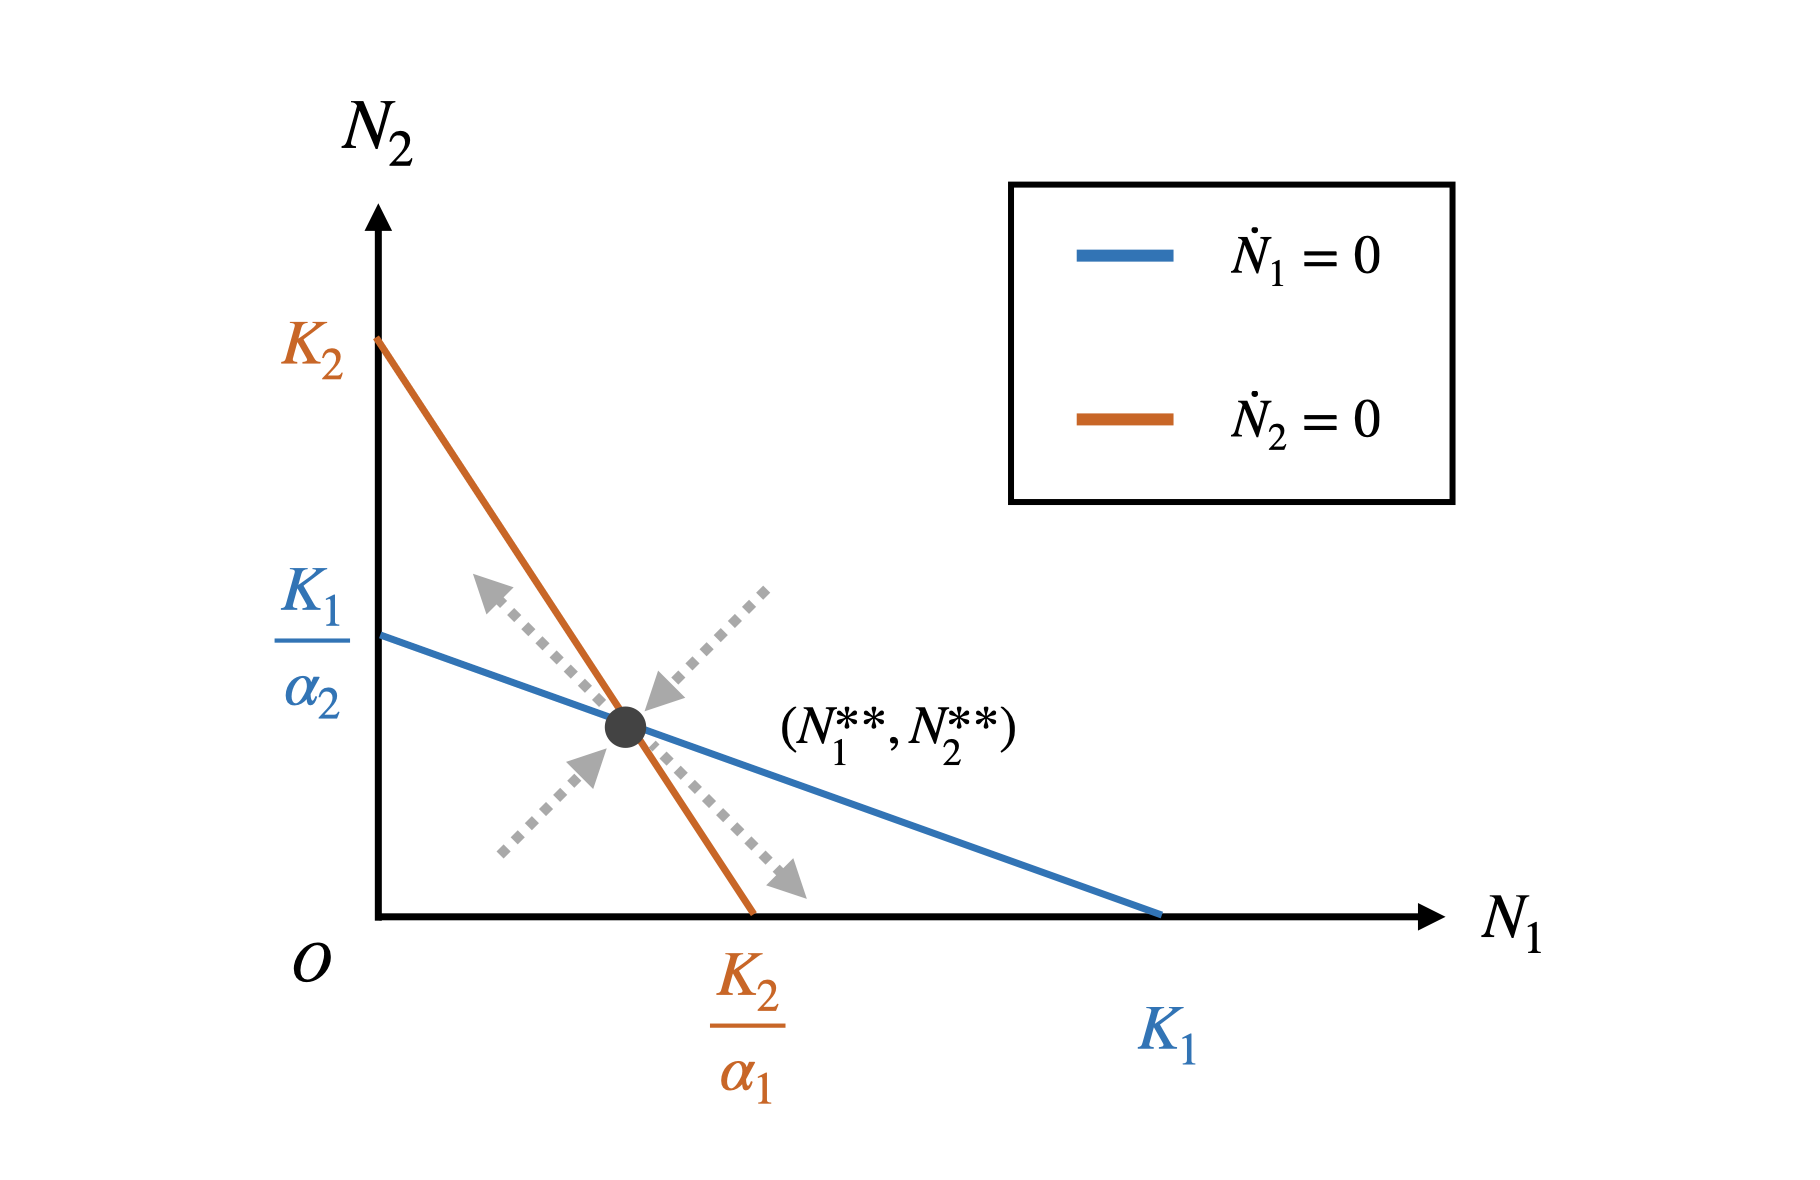
\includegraphics[width = \textwidth]{fig/graph_003.png}
  \caption {Vector space around the equilibrium in the Lotka-Volterra model when Equation \ref{equ:constraints} is met, derived from Figure \ref{fig:vecspace} . The dotted gray arrows indicate the direction of the vector after combining the previous 2 arrows.}
  \label{fig:equilibrium_stability}
\end{figure}

As we can see from the figure, the equilibrium is a saddle point, where it is stable in one axis and unstable in its orthogonal axis.
